\documentclass[11pt]{article}
\usepackage[margin=1in]{geometry}
\usepackage{graphicx}
\usepackage{booktabs}
\usepackage{amsmath}
\usepackage{xcolor}
\usepackage{listings}
\usepackage{float}
\usepackage[colorlinks=true,urlcolor=blue,linkcolor=black,citecolor=black]{hyperref}
\usepackage{caption}
\captionsetup{font=small,labelfont=bf}
\lstset{basicstyle=\ttfamily\small, breaklines=true, columns=fullflexible, frame=single,
        framerule=0.3pt, rulecolor=\color{gray}, xleftmargin=2pt, xrightmargin=2pt}
\setlength{\parskip}{0.45em}
\setlength{\parindent}{0pt}
\setlength{\emergencystretch}{3em}
\graphicspath{{../results/figures/}}

\title{MinHash for Efficient Agent Trajectories\\[0.3em]
\large COMP 480/580 --- Assignment 2}
\author{Aiden Vierra}
\date{December 2026}
\usepackage{titling}
\setlength{\droptitle}{-5em}

\begin{document}
\maketitle
\vspace{-2.5em}

\section{Overview}

We added two MinHash-based optimizations to the Spartacus agent harness and measured them
against the unmodified agent with each dataset's own \texttt{verify.py}:

\begin{itemize}
  \item \textbf{Task-level reuse} answers an incoming task from a previously verified one
        without running the agent, when the two are safely the same item.
  \item \textbf{Content-level reuse} replaces a tool output that nearly repeats an earlier
        one with a reference to it plus the exact lines that differ.
\end{itemize}

\textbf{Datasets (8 of 10):} \texttt{tickets}, \texttt{bugs} (record-based) and
\texttt{hosts}, \texttt{configs}, \texttt{code}, \texttt{threads}, \texttt{revisions},
\texttt{logs} (corpus-based). All six corpus datasets were kept because content-level reuse
can only act on them; \texttt{docs} and \texttt{citations} were left out of the live runs.
The code supports all ten, and the offline threshold sweep was checked on all ten.

\textbf{Model and harness:} \texttt{gemini-3.5-flash-lite} through OpenRouter, the same
model, prompt, tools and turn limit in every configuration. The implementation is three
files (\texttt{minhash.py}, \texttt{policy.py}, \texttt{content.py}) plus an experiment
runner (\texttt{run.py}) and analysis script (\texttt{plots.py}); neither Spartacus nor the
datasets were modified, and no code reads \texttt{hidden/}.

\textbf{Headline result.} Task-level reuse answered 13 of 64 sampled tasks (20\%) with
\emph{zero incorrect reuses}, each in under 10\,ms instead of about 21\,s and 113k input
tokens. Content-level reuse was correct but saved little in live runs (about 1.4\% of input
tokens), because the agent rarely re-reads near-duplicate files in full; offline, the same
layer shrinks a full read of a scenario to 26--43\% of its size on four of the six corpus
datasets.

\textbf{Git Repo:} \href{https://github.com/aidenvierra/comp480-assignment-2}{comp480-assignment-2}

\section{Implementation and Methodology}

\subsection{MinHash and LSH (\texttt{minhash.py})}

A text is lower-cased and split into alphanumeric tokens; its set of shingles is every run of
three consecutive tokens. Each shingle is hashed to a 32-bit integer $x$ with BLAKE2b, and
128 universal hash functions
\[
  h_i(x) = (a_i x + b_i) \bmod p, \qquad p = 2^{61}-1,\quad a_i, b_i < 2^{32},
\]
with $a_i, b_i$ drawn from a generator seeded with 480, give the signature
$s_i = \min_{x \in S} h_i(x)$. Because $x, a_i, b_i < 2^{32}$, $a_i x + b_i$ never overflows
a 64-bit integer, so the whole signature is one vectorized NumPy expression (about 4\,ms for
3\,000 shingles). The Jaccard estimate is the fraction of equal components,
$\hat J(A,B) = \frac{1}{128}\sum_i [s_i(A) = s_i(B)]$.

For retrieval, the signature is split into 32 bands of 4 rows; items that agree on any whole
band share a bucket and become candidates. With $b=32$, $r=4$ the probability of becoming a
candidate, $1-(1-J^4)^{32}$, crosses 50\% near $J = (1/32)^{1/4} \approx 0.42$, below every
threshold we use, so LSH only prunes and the threshold decides.

For content similarity an option masks numbers and hex identifiers to \texttt{0} before
shingling, so two host snapshots that differ only in values are recognised as near-copies.
Task similarity keeps digits, because \texttt{E-1042} and \texttt{E-1043} are different
tasks.

\subsection{Task-level reuse policy (\texttt{policy.py})}

The store for a dataset starts with every record of \texttt{history.jsonl}; a newly generated
answer is added only after it passes \texttt{verify.py}. An incoming task is answered from
the store only if a candidate passes \textbf{all three} of these checks; otherwise the agent
runs.

\begin{enumerate}
  \item \textbf{Similarity.} $\hat J \ge \tau$ on the dataset's similarity text
        (subject and body for tickets and corpus requests; title, body and stack trace for
        bugs).
  \item \textbf{Validation key.} The fields that each dataset's \texttt{INSTRUCTIONS.md} says
        must match, normalized exactly as stated there: (product, error code, platform) for
        tickets with \texttt{E-1042}\,=\,\texttt{e1042}; (exception, top frame, version
        series) for bugs; (scenario, kind, target) for every corpus dataset; (identifier,
        status class) for docs; the five graded fields for citations. A task whose key cannot
        be computed is never reused.
  \item \textbf{Decisive words.} The words that decide the answer are parsed at runtime
        from \texttt{INSTRUCTIONS.md}: the cue phrases of the ticket resolution guide
        (``story mentions \emph{clock}'') and the status words of the docs categories. If any
        of these words appears in one text but not the other, the match is rejected.
        Phrases are compared word by word, so a reworded cue still counts.
\end{enumerate}

Among candidates that pass, the most similar wins. An unknown dataset never reuses.

\textbf{Why this order.} Similarity cannot be the safety mechanism: on these datasets hard
negatives reach $\hat J = 1.00$ while true paraphrase duplicates sit at 0.15--0.37
(Section~\ref{sec:q2}). The key and the decisive words carry the safety; the similarity
threshold only controls how far from an exact copy we are willing to go.

\textbf{Threshold.} $\tau$ is set without labels. It starts at 0.5 and is raised above the
most similar pair of \emph{history} records that pass checks 2 and 3 yet have different
answers (a pair that the checks alone would wrongly merge), plus a 0.05 margin, capped at
0.9. On all eight datasets no such pair exists, so $\tau = 0.5$ everywhere. The sweep in
Section~\ref{sec:q3} that uses the verifier is analysis only and never feeds back into the
policy.

\subsection{Content-level reuse (\texttt{content.py})}

\texttt{read\_file}, \texttt{bash} and \texttt{grep} are replaced, through Spartacus's
\texttt{extra\_tools}, by same-named wrappers that call the original tool and pass its
output through a per-task cache. For each output of at least 400 characters:

\begin{enumerate}
  \item An \textbf{exact repeat} of an earlier output becomes
        \texttt{[reuse] identical to <earlier ref>}.
  \item Otherwise, if LSH finds an earlier output with masked-number $\hat J \ge 0.8$, a
        \textbf{line diff on the raw text} is computed and the agent receives
\begin{lstlisting}
[reuse] same as inventory/worker-01.txt except (17 of 97 lines differ):
L5: hostname = worker-02
L15: uptime_days = 23
L62: /  /dev/nvme0n1p2  ext4  size_gb=80  used_pct=87
\end{lstlisting}
        Similarity ignores digits, but the diff does not, so every changed number, identifier
        and configuration value is shown. The fold is used only if it is at most half the
        length of the original.
  \item A run of quoted e-mail lines (\texttt{> }) whose text appears verbatim in an
        earlier output becomes one reference line.
  \item Otherwise the original output is returned unchanged.
\end{enumerate}

Two rules keep references safe: they only point at an output the agent was shown in full
(never at another fold), and a request the agent repeats gets its full output. The second
rule came from a live failure: the agent re-read a file that had been shown as a diff,
received a pointer to that same file, and looped until the turn limit. The
\texttt{INSTRUCTIONS.md} of every corpus dataset already tells the agent how to read
\texttt{[reuse]} results, so prompts are identical across configurations.

\subsection{Harness integration and measurement}

\texttt{run.py} gives each task a fresh directory with only what the agent may see
(instructions, history, \texttt{task.json} and, for corpus tasks, that scenario's files),
runs the harness, grades \texttt{answer.json} with \texttt{verify.py}, and logs tool calls,
model requests, input and output tokens, wall time, and the time spent inside the policy and
the content cache. Wall time covers the whole task including MinHash work. Tasks within a
dataset run in stream (\texttt{seq}) order, so the store only ever holds earlier tasks.

Spartacus has no OpenRouter backend, so the runner points its OpenAI-compatible backend at
OpenRouter and makes two adjustments at the wire, without editing Spartacus:
\begin{itemize}
  \item Tool results are sent as \texttt{\{"result": text\}}, the shape Spartacus's native
        Gemini backend uses. Sent as raw text, OpenRouter forwarded only a JSON object found
        inside it: a read of \texttt{INSTRUCTIONS.md} reached the model as its example answer
        \texttt{\{"resolution\_id": "R-07"\}} and nothing else.
  \item When Gemini returns \texttt{MALFORMED\_FUNCTION\_CALL} (reproducible for a given
        conversation, no tokens billed), that request is retried with
        \texttt{tool\_choice: required}.
\end{itemize}
Sub-agents are disabled in all four configurations, because a spawned child agent would
bypass the content wrappers.

\section{Experimental Setup}

Each configuration ran on the same 64 tasks: a random sample of 8 incoming tasks per dataset
(seed 480), solved in stream order. A sample rather than the full stream was used to stay
within a \$10 API budget; a random sample was preferred over the first 8 tasks because
duplicates cluster later in each stream (the first 8 contain 7 reusable tasks, a random 8
contain 12--13). The four configurations are \textbf{baseline}, \textbf{task} (task-level
reuse only), \textbf{content} (content-level only) and \textbf{both}. Prices of \$0.30 and
\$2.50 per million input and output tokens give a total spend of about \$8.25, including a
16-task smoke run.

Each configuration was run once. With 8 tasks per dataset, run-to-run variance of the agent
is large compared with some of the effects measured, so Section~\ref{sec:results} also gives
\emph{attributable} savings that do not depend on comparing two noisy runs.

\section{Results}\label{sec:results}

\begin{table}[H]
\centering\footnotesize\setlength{\tabcolsep}{4pt}
\begin{tabular}{lrrrrrrr}
\toprule
Config & Acc.\,(\%) & Reused\,(\%) & Tool calls & Requests & Input tokens & Wall (s) & Overhead (ms) \\
\midrule
baseline & 96.9 & 0.0 & 11.4 & 12.4 & 94.8k & 21.8 & 0.0 \\
task & 96.9 & 20.3 & 9.8 ($-$13\%) & 10.6 ($-$14\%) & 80.7k ($-$15\%) & 18.7 ($-$14\%) & 2.3 \\
content & 95.3 & 0.0 & 10.3 ($-$9\%) & 11.3 ($-$8\%) & 69.6k ($-$27\%) & 19.1 ($-$12\%) & 15.0 \\
both & 95.3 & 20.3 & 8.9 ($-$21\%) & 9.7 ($-$21\%) & 79.6k ($-$16\%) & 16.2 ($-$26\%) & 15.5 \\
\bottomrule
\end{tabular}
\caption{Means per task over the same 64 tasks (8 per dataset). Overhead is the time spent in
MinHash lookup, indexing and content processing, and is included in wall time.}
\label{tab:overall}
\end{table}

\begin{table}[H]
\centering\small
\begin{tabular}{lrrrrrrrrr}
\toprule
 & \multicolumn{4}{c}{Passed (of 8)} & \multicolumn{4}{c}{Input tokens per task (k)} & Reused \\
\cmidrule(lr){2-5}\cmidrule(lr){6-9}
Dataset & base & task & cont. & both & base & task & cont. & both & (task) \\
\midrule
tickets & 8 & 8 & 8 & 7 & 90 & 89 & 80 & 89 & 1 \\
bugs & 8 & 8 & 7 & 7 & 207 & 141 & 131 & 135 & 3 \\
hosts & 8 & 8 & 8 & 8 & 68 & 40 & 40 & 47 & 2 \\
configs & 8 & 8 & 8 & 8 & 31 & 37 & 33 & 39 & 3 \\
code & 8 & 8 & 8 & 8 & 76 & 50 & 47 & 71 & 2 \\
threads & 7 & 8 & 8 & 8 & 68 & 73 & 77 & 79 & 1 \\
revisions & 7 & 6 & 6 & 7 & 148 & 152 & 87 & 112 & 1 \\
logs & 8 & 8 & 8 & 8 & 70 & 63 & 62 & 65 & 0 \\
\midrule
all & 62 & 62 & 61 & 61 & 95 & 81 & 70 & 80 & 13 \\
\bottomrule
\end{tabular}
\caption{Per-dataset accuracy and input tokens.}
\label{tab:datasets}
\end{table}

\textbf{Correctness.} No reused answer failed verification, in either configuration with
task reuse. Every failure was inspected: none was caused by a reuse decision, and none by a
fold hiding information (replaying each trajectory through the content cache shows the folds
were lossless). The 1--2 task differences in accuracy between configurations are run-to-run
variance; for example, \texttt{revisions} task \texttt{T-3c0fab} failed in three
configurations with different wrong answers and no folds.

\textbf{Attributable savings.} Two estimates that do not rely on comparing separate runs:
\begin{itemize}
  \item \emph{Task-level.} The 13 reused tasks cost the baseline 1.48M input tokens, 142 tool
        calls and 274\,s, which is \textbf{24\%} of all baseline input tokens and
        \textbf{20\%} of its tool calls and wall time. Reuse replaced each with an 8\,ms
        lookup.
  \item \emph{Content-level.} Replaying every content-configuration trajectory and weighting
        each saved character by the number of later model requests that re-send it gives
        about 64k tokens, \textbf{1.4\%} of that configuration's input tokens (7.2\% on
        \texttt{code}, 3.2\% on \texttt{revisions}, under 2\% elsewhere). The content
        configuration's raw 27\% reduction in Table~\ref{tab:overall} is mostly variance in
        the agent's path, not the folds.
\end{itemize}

\begin{figure}[tbp]
\centering
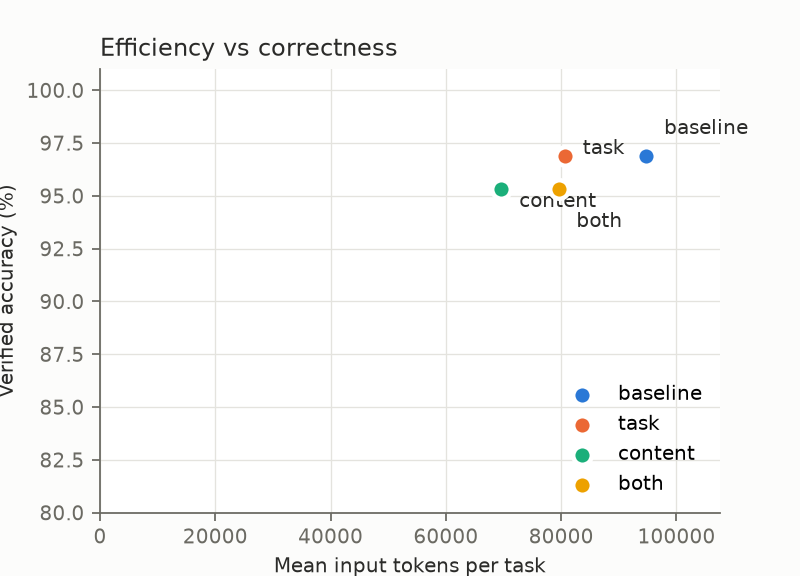
\includegraphics[width=0.5\linewidth]{efficiency_vs_accuracy.png}
\caption{Efficiency vs.\ correctness: mean input tokens per task and verified accuracy for
each configuration.}
\label{fig:eff}
\end{figure}

\begin{figure}[tbp]
\centering
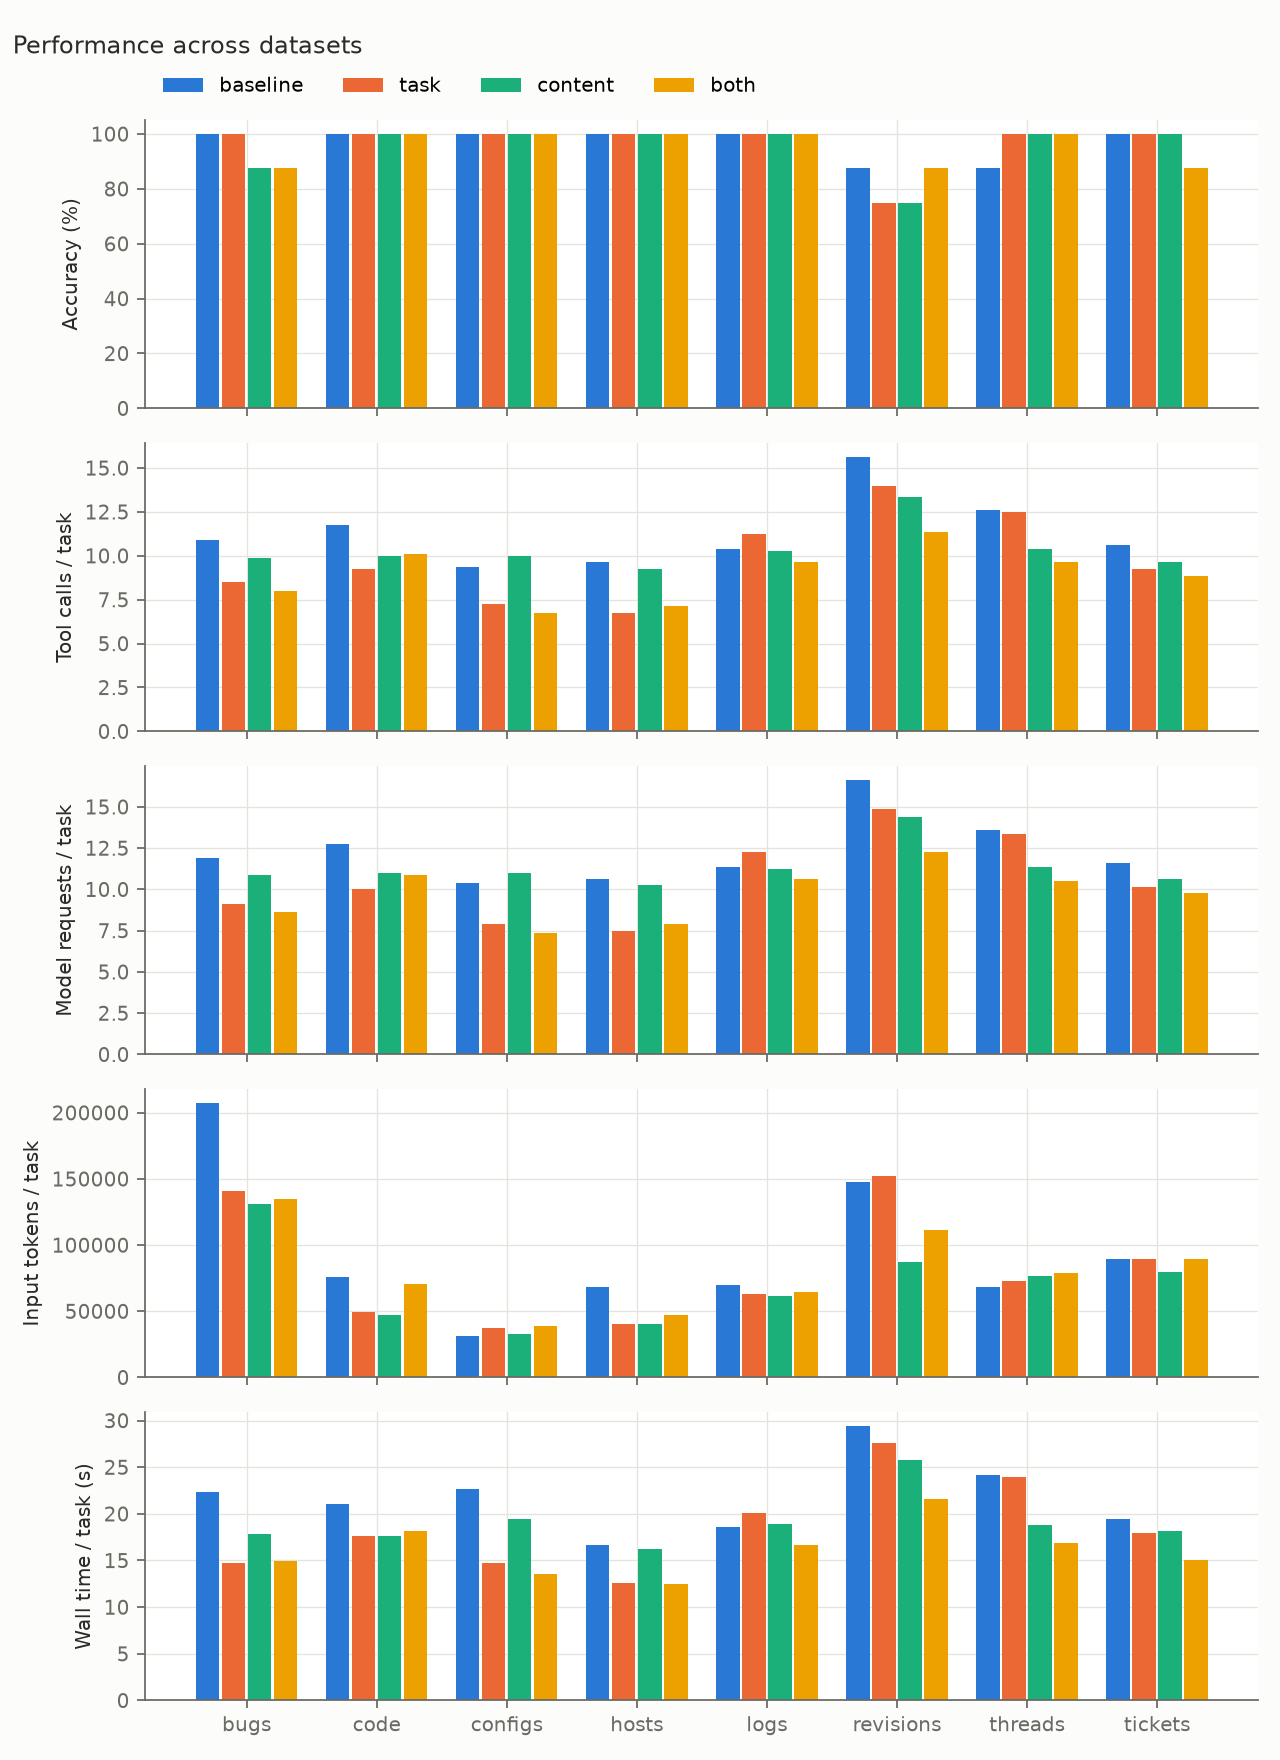
\includegraphics[width=0.62\linewidth]{per_dataset_metrics.png}
\caption{Performance across datasets: accuracy, tool calls, model requests, input tokens and
wall time per task.}
\label{fig:datasets}
\end{figure}

\begin{figure}[tbp]
\centering
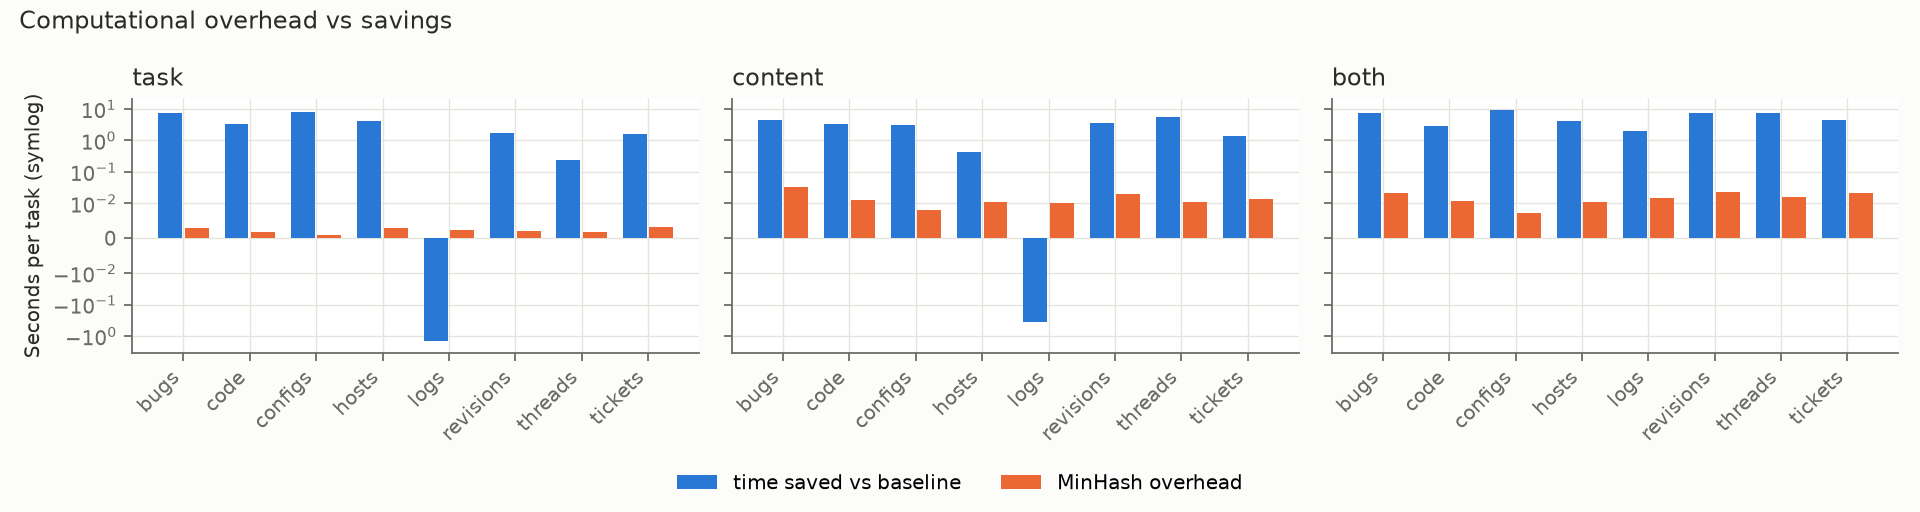
\includegraphics[width=\linewidth]{overhead_vs_savings.png}
\caption{Computational overhead vs.\ savings per task (symmetric log scale). MinHash overhead
is milliseconds; savings are seconds.}
\label{fig:overhead}
\end{figure}

\section{Discussion}

\subsection{When is task reuse beneficial?}

Task reuse pays off whenever a task is a re-submission of an item that was already solved
and verified, because then \emph{no agent execution is needed at all}: no model requests, no
tool calls, no tokens. In our runs the 13 reused tasks would have cost the baseline 113k
input tokens, 11 tool calls and 21\,s each; reuse answered them in 8\,ms. The benefit is
largest where the agent's own work is most expensive: on \texttt{bugs}, where the agent reads
a 120k-character history file, three reuses cut that dataset's input tokens by a third.

The tasks best suited to MinHash reuse are those whose duplicates keep most of their wording:
exact copies, reformatted copies, reordered paragraphs and lightly edited versions with typos.
Per each dataset's \texttt{MANIFEST.json} these start at $\hat J$ 0.54--0.73 (edits) and reach
1.0 (exact and reformatted copies); they are the ones that were reused.
Task reuse can eliminate execution entirely only when \emph{everything that decides the
answer} is visible and checkable in the task itself: structured fields (scenario, kind,
target; product, code, platform) plus a small vocabulary of answer-deciding words. Corpus
requests are the cleanest case: (scenario, kind, target) fully determines the answer, so a
verified match needs no further work. Duplicates of earlier \emph{incoming} tasks are also
reusable once the earlier answer has been verified; in the combined run
\texttt{tickets/T-fc2c7e} was answered from the verified answer of \texttt{T-e65487}.

\subsection{Is high similarity sufficient for safe reuse?}\label{sec:q2}

No. In every dataset the most similar wrong match is almost a copy:

\begin{itemize}
  \item \texttt{logs}: \texttt{T-139e21} and history \texttt{H-755b0d} have $\hat J = 1.00$.
        Both ask for the drifted host, word for word, but about different incidents
        (\texttt{INC-1076} vs.\ \texttt{INC-1684}), so the answers differ.
  \item \texttt{hosts}: \texttt{T-45d76f} vs.\ \texttt{H-219cd0}, $\hat J = 0.99$, the same
        ``which host has a service that is not running'' about fleets \texttt{FLT-1684} and
        \texttt{FLT-1152}. Reusing would answer \texttt{worker-06}/\texttt{node-exporter} for
        the wrong fleet.
  \item \texttt{tickets}: \texttt{T-07ab1c} vs.\ \texttt{H-d1018e}, $\hat J = 0.96$, the same
        TLS-inspection story on Android and macOS; the resolution guide has a platform
        exception, so the answers differ.
\end{itemize}

Each of these is rejected by the validation key. The decisive-word check handles the harder
case where the key matches. \texttt{tickets/T-e01fd5} and history \texttt{H-ae3ecd} share
product, error code (\texttt{E-3307}) and platform, and $\hat J = 0.58$, but the stories
differ: ``yesterday's plan upgrade is not reflected'' (cue \emph{plan change},
\texttt{R-02}) vs.\ ``a duplicate import run doubled every record'' (cue \emph{duplicate
batch}, \texttt{R-21}). Our first version matched cue phrases whole, saw neither phrase, and
reused \texttt{R-21}; the offline sweep caught the wrong reuse. Comparing cue words
individually (``duplicate'' appears in one text only) rejects it.

Across all 370 incoming tasks of the 8 datasets at $\tau = 0.5$, similarity alone reuses 204
answers of which \textbf{116 are wrong}; the full policy reuses 80 with \textbf{none wrong}.
Even at $\tau = 1.0$, similarity alone makes 2 wrong reuses. In the live task configuration,
the reasons for not reusing were: key mismatch 26 times, no candidate 19, below threshold 4,
decisive-word mismatch 2.

\subsection{How does the similarity threshold affect performance?}\label{sec:q3}

\begin{figure}[tbp]
\centering
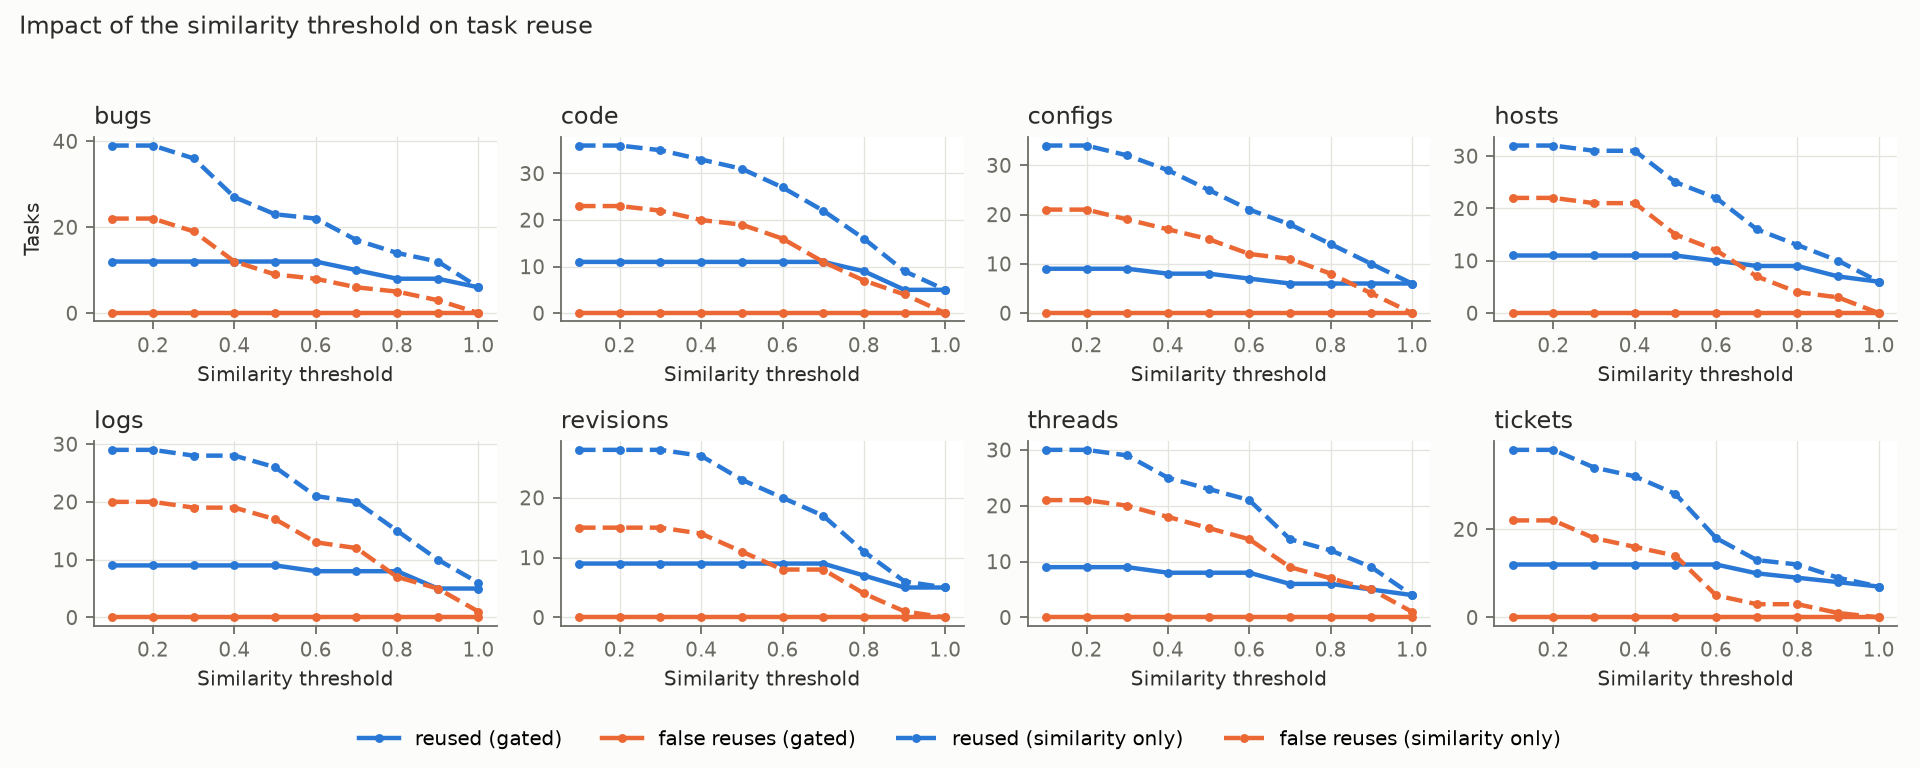
\includegraphics[width=\linewidth]{threshold_sweep.png}
\caption{Impact of the similarity threshold (offline, all incoming tasks against history,
each reuse scored by \texttt{verify.py}). Solid: full policy; dashed: similarity only.}
\label{fig:sweep}
\end{figure}

\begin{table}[H]
\centering\small
\begin{tabular}{lrrrrrr}
\toprule
$\tau$ & 0.3 & 0.5 & 0.7 & 0.8 & 0.9 & 1.0 \\
\midrule
Full policy: reused / wrong & 82 / 0 & 80 / 0 & 69 / 0 & 62 / 0 & 49 / 0 & 44 / 0 \\
Similarity only: reused / wrong & 253 / 153 & 204 / 116 & 137 / 67 & 107 / 45 & 75 / 26 & 45 / 2 \\
\bottomrule
\end{tabular}
\caption{Threshold sweep totals over 370 tasks in 8 datasets.}
\label{tab:sweep}
\end{table}

For similarity-only reuse the threshold is a straight trade between duplicates found and hard
negatives merged: lowering $\tau$ from 0.9 to 0.5 finds 129 more matches, but 90 of them are
wrong. No threshold is safe, because hard negatives (0.41--0.95 in the manifests, and up to 1.00
for a same-worded request about another scenario) overlap the duplicates we want (0.54--1.0)
and sit above paraphrases (0.15--0.37).

With validation, the threshold stops being a safety parameter and becomes a recall
parameter: false reuses stay at zero at every $\tau$, and lowering $\tau$ from 1.0 to 0.5
nearly doubles the reuses (44 to 80). Below 0.5 almost nothing is gained (82 at 0.3), since
the remaining duplicates are paraphrases whose similarity is near that of unrelated tasks.

A single \emph{similarity-only} threshold would not suit every dataset: the most similar
hard negative ranges from 0.80 (\texttt{tickets}) to 0.95 (\texttt{bugs}) in the manifests,
while edit duplicates start between 0.54 (\texttt{logs}) and 0.73 (\texttt{hosts}), so each
dataset would need its own compromise and none would be free of wrong reuses. With
validation a single threshold of 0.5 is appropriate for all eight datasets, and our
history-based calibration found no reason to raise it anywhere. On a dataset whose
validation rule were weaker (fields necessary but further from sufficient), the calibration
would raise $\tau$ for that dataset alone.

\subsection{When is content-level reuse effective?}

Content reuse is effective when the agent reads many near-identical outputs \emph{in full}
and the differences are a small share of each. Reading every file of every scenario offline,
the layer reduces the text to 26\% (\texttt{code}: one template copied into each payment
adapter), 37\% (\texttt{configs}), 40\% (\texttt{hosts}) and 43\% (\texttt{revisions}) of its
size, in 4--5\,ms per scenario. In the live runs the largest attributable savings were on
\texttt{code} (7.2\% of input tokens) and \texttt{revisions} (3.2\%), where the agent did
read several adapters or revisions one after another, for example \texttt{policy/v07.md}
folded to 8 changed lines of \texttt{v01.md} (2\,173 to 827 characters).

The same approach gives nothing on \texttt{logs}: two hosts' logs are near-identical up to
numbers (masked $\hat J$ 0.96--1.00), but every line carries its own timestamp and request
id, so the exact diff is as long as the file and the layer declines every fold. A masked
diff would be shorter but would hide the drifted \texttt{pool\_size=32} that some tasks ask
for. On \texttt{threads} replies differ by whole new bodies, so only quoted blocks fold
(82\% offline). And in live runs the benefit is small everywhere, because the agent mostly
uses \texttt{grep} or reads two or three files rather than every near-duplicate; the record
datasets give the layer almost nothing to fold.

\subsection{Which optimization is more valuable?}

On these workloads, \textbf{task-level reuse}:

\begin{itemize}
  \item \emph{Correctness:} both preserved accuracy. Task reuse has a sharper failure mode
        (a wrong reuse is a wrong answer), which the validation checks prevent; content
        reuse cannot answer wrongly by itself, since every fold is lossless.
  \item \emph{Token savings:} task reuse removed 24\% of baseline input tokens attributably,
        content reuse about 1.4\%.
  \item \emph{Tool calls and completion time:} a reused task needs no tool calls and finishes
        in milliseconds, removing about 20\% of baseline tool calls and wall time. Content
        reuse does not remove tool calls (the agent still makes the call) and saves only the
        re-sent tokens.
\end{itemize}

We would prefer task reuse whenever the stream repeats items and the answer is fully
determined by fields that can be validated: support queues, triage, repeated questions about
the same environment. Content reuse is preferable when tasks are new each time but the
environment is repetitive and the agent must read much of it: many near-identical configs,
code copied from a template, successive document versions. The two are complementary: in the
combined configuration tool calls fell 21\% and wall time 26\%, the largest drops of the
four, though at this sample size that ordering is within noise.

\subsection{What are the limitations of MinHash for agents?}

\textbf{Lexical similarity is not task equivalence.} It misses true duplicates that are
reworded: paraphrases share only 15--37\% of their shingles and are never reused, so every
paraphrase still costs a full agent run. It also matches non-duplicates that share almost all
of their wording: a request about another scenario or platform, or a story with one changed
cue, sits at 0.6--1.0. Only the dataset-specific validation keeps those out, and that rule
had to be written per dataset from its instructions; a new dataset without one gets no task
reuse at all.

\textbf{Overhead can exceed savings.} Here it never did: lookup and indexing take about
2\,ms per task and content processing about 15\,ms, against 20\,s agent runs. It would when
no reuse is possible and outputs are large: on \texttt{logs} the content layer hashed and
diffed about 9.5\,ms per scenario and folded nothing. With cheap tasks (a few hundred tokens)
or very large stores the fixed cost of signatures and diffs approaches the cost of simply
running the model, and content folds can even cost tokens when the agent re-reads a file to
reconstruct what a fold left out.

\textbf{One improvement.} Use semantic embeddings for candidate retrieval and keep the
validation checks as the safety gate. Embeddings would recognise paraphrased duplicates that
MinHash misses (the largest group of missed reuses here), while the structured key and
decisive-word checks continue to reject the hard negatives that any similarity measure,
lexical or semantic, will score highly.

\subsection{Limitations of this study}

Each configuration ran once on 8 tasks per dataset to stay within budget, so per-dataset
differences of a task or two are not significant; the attributable-savings estimates above
are the more reliable comparison. Content reuse was measured with the agent's own reading
strategy; an agent that reads whole directories would benefit more, as the offline numbers
show.

\appendix
\section{Reproducing the experiments}

\begin{lstlisting}
git clone https://github.com/sahiljoshi515/Spartacus
git clone https://github.com/aidenvierra/comp480-assignment-2.git Assignment2_COMP_580
python3 -m venv .venv && .venv/bin/pip install -r requirements.txt
echo 'OPENAI_API_KEY=<openrouter key>' >> ~/.config/spartacus/env

.venv/bin/python -m unittest test_minhash                 # offline tests
.venv/bin/python plots.py sweep --out results/sweep.csv   # no API calls
for c in baseline task content both; do
  .venv/bin/python run.py --config $c --out results/full --jobs 8 --trace --cap 9
done
.venv/bin/python plots.py report --results results/full \
    --out results/figures --sweep results/sweep.csv
\end{lstlisting}

Defaults: 8 tasks per dataset sampled with seed 480 and solved in \texttt{seq} order; MinHash
seed 480; LSH 32 bands $\times$ 4 rows; task threshold calibrated per dataset (0.5 on all
eight); content threshold 0.8, minimum output 400 characters, folds used only at
$\le 50\%$ of the original. A rerun skips tasks already logged, and \texttt{--fake} runs the
whole pipeline with a stub model at no cost.

\end{document}
